% Source of Figure 1 (fig_comb.pdf). Compile with: pdflatex fig_comb
\documentclass[border=2pt]{standalone}
\usepackage[T1]{fontenc}
\usepackage{mathptmx}
\usepackage{xcolor}
\usepackage{tikz}
\usetikzlibrary{arrows.meta}
\definecolor{cblue}{HTML}{2A78D6}
\definecolor{corange}{HTML}{EB6834}
\definecolor{caqua}{HTML}{1BAF7A}
\definecolor{cgray}{HTML}{8A8984}
\begin{document}
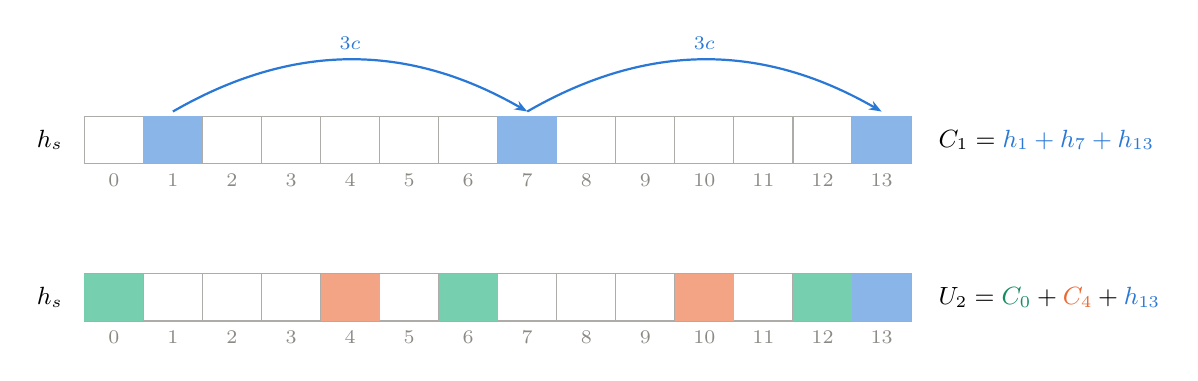
\begin{tikzpicture}[x=7.5mm,y=6mm,every node/.style={font=\small}]
  \foreach \s in {0,...,13}{\draw[cgray!70] (\s,0) rectangle (\s+1,1); \node[font=\scriptsize,cgray] at (\s+0.5,-0.35) {\s};}
  \node[anchor=east] at (-0.2,0.5) {$h_s$};
  \foreach \s in {1,7,13}{\fill[cblue!55] (\s,0) rectangle (\s+1,1);}
  \draw[cblue,thick,-{Stealth[length=1.6mm]}] (1.5,1.1) to[bend left=30] node[above,font=\scriptsize]{$3c$} (7.5,1.1);
  \draw[cblue,thick,-{Stealth[length=1.6mm]}] (7.5,1.1) to[bend left=30] node[above,font=\scriptsize]{$3c$} (13.5,1.1);
  \node[anchor=west] at (14.3,0.5) {$C_1=\textcolor{cblue}{h_1+h_7+h_{13}}$};
  \begin{scope}[yshift=-20mm]
  \foreach \s in {0,...,13}{\draw[cgray!70] (\s,0) rectangle (\s+1,1); \node[font=\scriptsize,cgray] at (\s+0.5,-0.35) {\s};}
  \node[anchor=east] at (-0.2,0.5) {$h_s$};
  \foreach \s in {0,6,12}{\fill[caqua!60] (\s,0) rectangle (\s+1,1);}
  \foreach \s in {4,10}{\fill[corange!60] (\s,0) rectangle (\s+1,1);}
  \fill[cblue!55] (13,0) rectangle (14,1);
  \node[anchor=west,align=left] at (14.3,0.5) {$U_2=\textcolor{caqua!80!black}{C_0}+\textcolor{corange}{C_4}+\textcolor{cblue}{h_{13}}$};
  \end{scope}
\end{tikzpicture}
\end{document}
